\chapter{Time-memory-data tradeoff using Hellman tables}
\label{chapter:tmdto-hellman}


\footnotesize
\indent \textbf{\textit{Summary.}} Time-memory tradeoff attacks were first conceived on block ciphers by Hellman in 1980. In this approach, Hellman proposed a method for carrying out the precomputation phase of the attack i.e. computing the precomputation tables. We refer to these tables as Hellman tables for block ciphers, in the remainder of the thesis. The proposed idea is based on the birthday paradox, and is thus probabilistic in nature, as we shall see in a moment. 

Later, using this approach as the basis, Shamir and Biryukov proposed a table structure for stream ciphers. This takes into account the amount of keystream available for the attack. We call these tables as Hellman tables for stream ciphers. We start by explaining the original idea of Hellman based on block ciphers. This is done by first presenting a naive approach to building tables for time-memory tradeoff attacks on block ciphers. Then, we point out limitations to the approach and explain how they are improved, consequently leading to the original idea of Hellman. From there, we provide the idea of Shamir and Biryukov, which is used for implementing a time-memory-data tradeoff attack on HiTag2 cipher.

\normalsize
\section{Hellman tables for block ciphers}

A block cipher is an encryption algorithm, which takes in a plaintext block of $n$ bits (called the block size) and a key of $k$ bits, and returns a ciphertext block of $n$ bits. Figure \ref{fig:block-cipher} illustrates a simple block cipher, with plaintext, ciphertext and key represented by $P$, $C$ and $K$ respectively. The encryption function is denoted by $E$ such that $C$ = $E_K(P)$ and implying encryption of $P$ under $K$.

\begin{figure}[ht!]
	\centering
		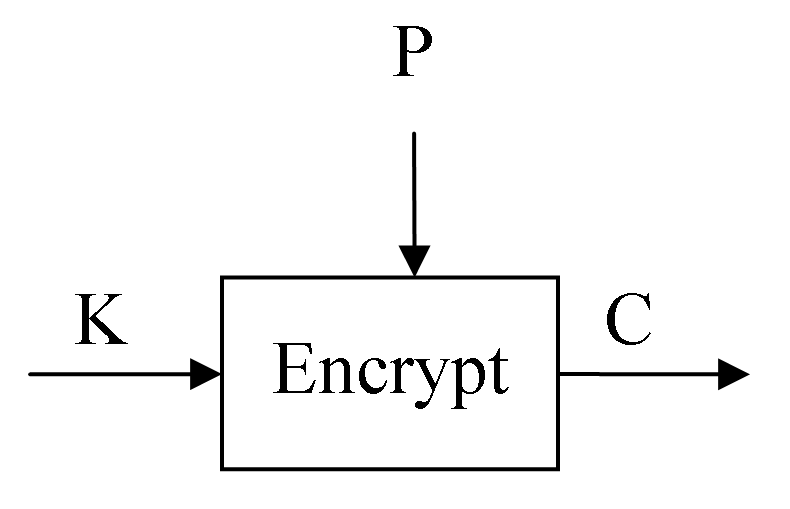
\includegraphics[width=2in]{./figures/block-cipher.PNG}
	\caption{A block cipher}	
	\label{fig:block-cipher}
\end{figure}

\subsection{The ideal TMTO attack}
Consider the following general scenario for a TMTO attack on block ciphers. The attacker has knowledge of a particular plaintext block $P$ and the corresponding ciphertext block $C$. The goal is to find $K$, using which the attacker can decipher ciphertext corresponding to unknown plaintext. In addition, for simplicity, we assume the size of $K$ to be equal to the block size of $n$ bits. Then following we have the precomputation and attack phases for the attack in an ideal case.\\

\noindent \textit{\textbf{Precomputation phase.}} An $n$ bit value is randomly selected using a uniform distribution (and denoted by $SP$ for a starting point). Using $SP$ as a key (denoted by $K_0$), encryption of $P$ is performed. The ciphertext obtained from this encryption is then used as the key (denoted by $K_1$) for the subsequent round of encryption of $P$. This procedure is iterated over a total of $t$ encryptions, yielding the key $K_t$ at the end. The key $K_t$ is called an end point, and is represented by $EP$. Moreover, the sequence of encryptions starting from $SP$ to $EP$ is called a \emph{chain} and is illustrated in the figure \ref{fig:block-cipher-single-chain}. Equations for the $t$ encryptions are also shown below. 

\begin{align*}
& & K_0 &= SP & & & &\\
1&. & K_1 &= E_{K_0}(P) & & & &\\
2&. & K_2 &= E_{K_1}(P) & & & &\\
& & &\vdots & & & &\\
(t-1)&. &K_{t-1} &= E_{K_{t-2}}(P) & & & &\\
(t)&. &K_{t} &= E_{K_{t-1}}(P) & & & &\\
& & EP &= K_{t} & & & &\\
\end{align*}

\begin{figure}[ht!]
	\centering
		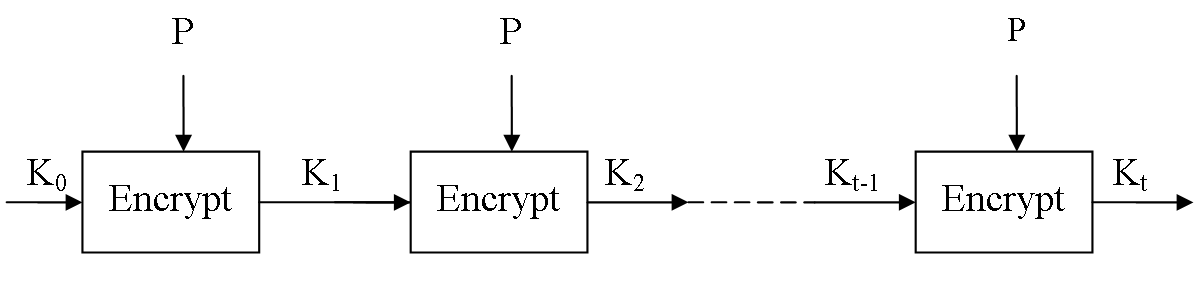
\includegraphics[width=5.5in]{./figures/block-cipher-single-chain.PNG}
	\caption{A chain of encryptions}	
	\label{fig:block-cipher-single-chain}
\end{figure}

During the precomputation phase, the goal is to cover the entire key space such that all possible keys exist in the table structure. A single chain covers a total of $t$ distinct keys. Though the chain contains a total of $(t+1)$ keys starting from $K_0$ to $K_{t}$, only the first $t$ keys are useful during the attack phase. This we shall explain later, and for the moment we note that only $t$ keys are represented in the chain.

\begin{figure}[ht!]
	\centering
		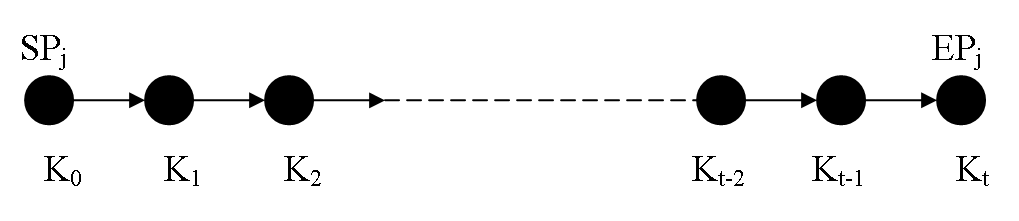
\includegraphics[width=4in]{./figures/single-chain.PNG}
	\caption{A single chain of encryptions represented by the pair $SP_j$ and $EP_j$}	
	\label{fig:single-chain}
\end{figure}

\begin{figure}[ht!]
	\centering
		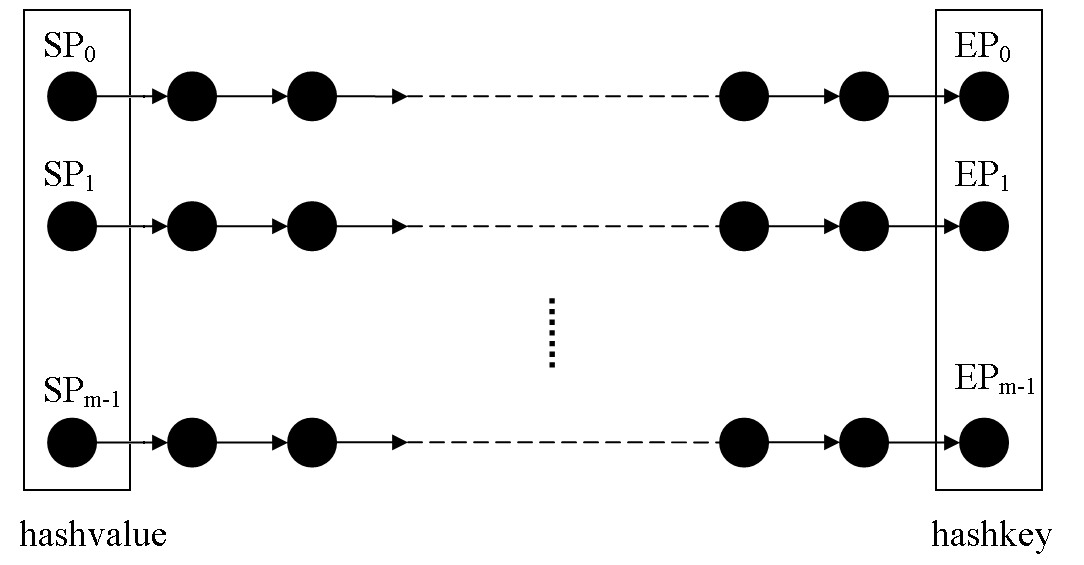
\includegraphics[width=4.5in]{./figures/naive-hellman-table.PNG}
	\caption{A naive precomputation table structure}	
	\label{fig:naive-hellman-table}
\end{figure}

An appropriate length $t$ of the chain is chosen so that no key repeats in the chain. Repetition is not desired since once a key reappears, subsequent keys would also repeat, adding no extra information to the chain. Hence, the size of the chain is restricted, and more than one chains are created instead. 

Lets say $m$ more such chains are needed to cover all possible keys. If we consider the ideal case in which each chain contains $k$ distinct keys, then we have $m$ = $2^n/t$. For each chain, we select a random starting point $SP_j$ and end up with the end point $EP_j$, for $1 \leq j \leq m$, as shown in figure \ref{fig:single-chain}. Only the pairs $(SP_j,EP_j)$ are then stored in a hashtable, with $EP_j$ as the key and $SP_j$ as the corresponding value. All the chains representing such a table structure are illustrated in the figure \ref{fig:naive-hellman-table}.

We now compute $M$ and $P$ for the precomputation phase. The size of the memory required for storing all the chains would be of the order of $m$, as there are $m$ chains and a constant number of elements ($SP$ and $EP$) corresponding to each chain are stored. Hence we have $M$ = $m$. Also, as there are $mt$ encryptions performed in the entire table, the precomputation time is give by $P$ = $mt$.\\

\noindent \textit{\textbf{Attack phase.}} If the required key $K$ exists in among the first $t$ keys in any chain, the ciphertext $C$ would also exist. The possible locations of $K$ in every chain are from $SP_j$ to $K_{j,t-1}$. $EP_j$ is not considered to be a possible key since it is not used in the encryption of $P$. Or in other words, the ciphertext obtained from $K_{j,t}$ is not computed and thus not stored in the chain, hence it cannot be matched with the available ciphertext $C$. So, there are $t$ possible values for $K$ per chain. Looking at this from the perspective of $C$, there are also $t$ possible values of ciphertext in every chain that can match with $C$. These $t$ possible matches correspond to each of the $t$ possible keys, and range from $K_{j,1}$ to $K_{j,t}$.

The first possibility is that $C$ lies in $t$'th column of any one of the $m$ chains. This is true only if $C$ equals some $EP_j$ stored in the hashtable. In such a case $K_{j,t-1}$ is the key we are looking for. To find this key, we retrieve $SP_j$ corresponding to $EP_j$ from the hashtable (by giving $EP_j$ as the key, we get the corresponding value $SP_j$), and perform $(t-1)$ encryptions on $P$ starting by $SP_j$ as the key (just in the same way as done during precomputation: using output of one encryption as key for next encryption). After $(t-1)$ encryptions, $K_{t-1}$ is obtained, which is the desired key. 

If $C$ does not match any of the $EP_j$, the next possibility is that $C$ lies in the $(t-1)$'th column of some chain. If this is indeed the case, then $X$ = $E_{C}(P)$ must match with some $EP_j$. On a match, we know that the key $K_{j,t-2}$ is the required key. To find out $K_{j,t-2}$, we retrieve $SP_j$ correspondng to the matched $EP_j$ and perform $(t-2)$ encryptions. If none of the $EP_j$ matches with the evaluated $X$, we explore the possibility of $C$ lying in the remaining columns, one by one.

If $C$ exists in the chains, then the time taken to find $K$ is actually the same as the length of each chain. Assuming $C$ exists in the $r$'th column (such that  $2 \leq r \leq t$, then $X$ is computed by performing $(t-r)$ encryptions in the following way.

\begin{align*}
& & K_r &= C & & & &\\
1&. &K_{r+1} &= E_{K_r}(P)  & & & &\\
2&. &K_{r+2} &= E_{K_{r+1}}(P) & & & &\\
& & &\vdots & & & &\\
(t-r) &. &K_{r + (t-r)} &= E_{K_{r + (t-r-1)}}(P) & & & &\\
& & X &= K_{r + (t - r)} & & & &\\
\end{align*}

If $X$ matches an $EP_j$, then $(r-1)$ encryptions are performed to retrieve the key $K_{r-1}$. In all, the number of encryptions performed is $(t-1)$. The attack time is of the order of $t$, thus our attack parameter $T$ = $t$. \\

\noindent \textit{\textbf{Problems with above approach.}} The approach described above is an ideal case, and some serious problems exist with it.

\begin{enumerate}

\item We have assumed that the length of $K$ is equal to the block size. This assumption does not hold for practical block ciphers, and thus we need to design a solution considering different key length and block size. Generally, the block size is larger than the key length. Thus a reduction function $R$ is required for the conversion of $n$ bits of $C$ to $k$ bits of $K$, provided $n > k$. 

% some example reduction functions

During precomputation phase, the encryption function is replaced with the new function, which performs encryption and reduction to give the new key. This function is called the \emph{mapping function} (denoted by $F$), since it maps one key to another in the same keyspace. Such a mapping function is shown in figure \ref{fig:mapping-function}. 

\begin{figure}[ht!]
	\centering
		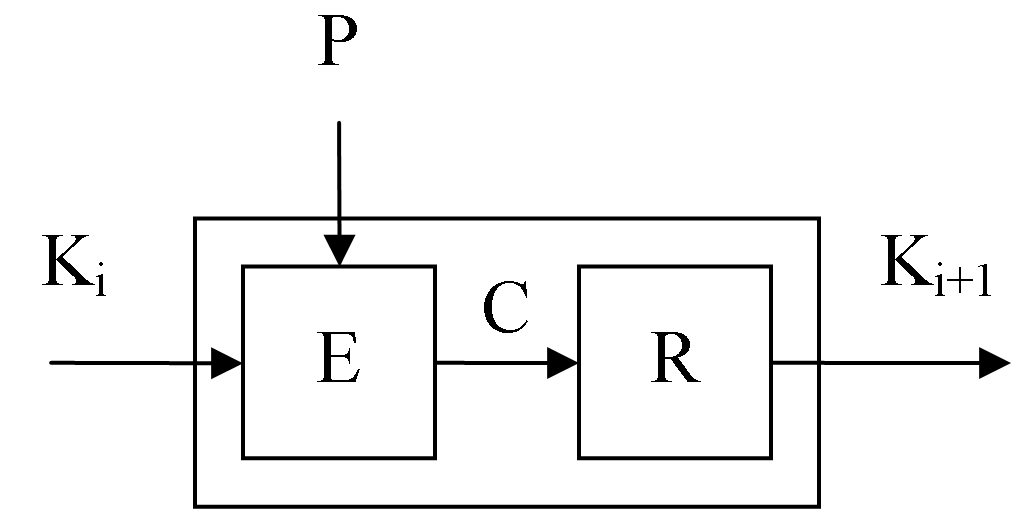
\includegraphics[width=3in]{./figures/mapping-function.PNG}
	\caption{Mapping function for block ciphers}	
	\label{fig:mapping-function}
\end{figure}

The function can also be represented in notation as follows, where $R$ stands for the reduction function.

\begin{center}
$K_{i+1}$ = $F(K_i)$ = $R(E_{K_i}(P))$\\
\end{center}

\item A much more serious problem in the ideal case is the assumption that all the possible keys exist in the table structure and that no key is repeated. It is desired that all keys are covered in some chain, but practically this is hard to achieve. The reason is that as more and more keys are covered in the table, repetition of keys becomes frequent after a certain time. The rate of repetitions grows exponentially from then on thus making it difficult to search and include new keys in the chains. This claim is actually justified using the variant of the birthday paradox.

Suppose so far we have $m$ chains with $t$ keys each. A new chain is then added to the table. The total number of keys existing in the table are $mt$ while $t$ more keys are added through the new chain. We are interested in restricting $m$ and $t$ so that there is no common key between the $m$ chains and the new chain. According to the variant of the birthday paradox, the product of the sizes of these two sets should be less than or equal to the space size, in order to have a high probability that no common element occurs. Then, we have 

\begin{center}
$mt \times t \leq 2^n$\\
$mt^2 \leq 2^n$\\
\end{center}

If the $<$ condition is removed, then we have an upper bound on the value of $mt^2$ called the \emph{table stopping rule} and represented by the condition 
$mt^2 = 2^n$. 

In the ideal case, all the keys are covered in the $m$ chains, hence we have $mt$ = $2^n$. If we use this equation in estimating the value of $mt^2$, it can be seen that $mt^2$ is much greater than $2^n$. This ofcourse is not allowed according to the table stopping rule, and thus extensive collisions are bound to take place in our ideal case. Repetition of keys gives rise to the problems of \emph{collision and merge} during the precomputation phase and \emph{false alarms} during the attack phase. We explain these two problems in detail below.
\end{enumerate}

\noindent \textit{\textbf{Collision and merge.}} Consider the first two chains in the precomputation table structure. If there is a common key $K_c$ between these chains, then the sequence of keys appearing (in both the chains) after $K_c$ would be the same, as shown in figure \ref{fig:collision-merge}. If the position where $K_c$ appears is the same in both the chains, then the end points of the chains is same. Otherwise, the end points are different. But irrespective of the position of the $K_c$, it can be clearly seen that there are overlapping keys in the two chains, resulting in wastage of precomputation time by adding no extra information.\\

\begin{figure}[ht!]
	\centering
		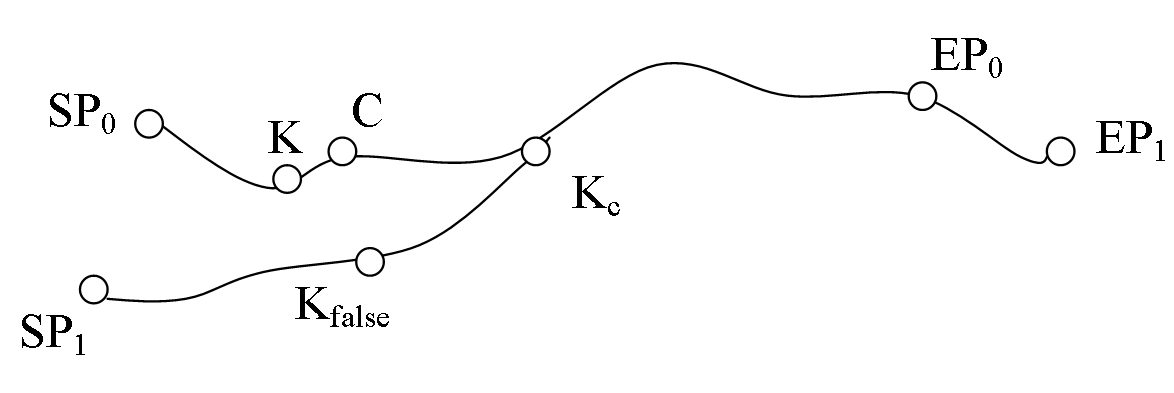
\includegraphics[width=4.5in]{./figures/collision-merge.PNG}
	\caption{Two chains which collide and consequently merge}	
	\label{fig:collision-merge}
\end{figure}

\noindent \textit{\textbf{False alarms.}} Colliding and merging chains during precomputation effect the attack phase as well. Consider the same example of the two chains colliding at $K_c$. Suppose that the required key $K$ appears in the first chain. During the attack phase keys are computed starting from $C$ till one of these keys matches some end point in the hashtable. 
In the example, a match would occur at $EP_0$ since $EP_0$ is one of the keys in the path from $C$ to $EP_1$ and $EP_0$ exists in the hashtable. The hashtable would return the starting point as $SP_0$ for the match, and thus a key is derived from $SP_0$ ($K_{false}$) which is different from the desired key $K$. It can be seen that $K$ lies in a different chain, but as the two chains collide and merge, the desired key not obtained from the the correct chain. A false alarm is said to have occured here.

The occurence of false alarms can be easily checked and ignored. It is expected that the ciphertext obtained by encrypting $P$ under the derived key be the same as $C$. If $K_{false}$ is used, the ciphertext obtained is not the same as $C$ as both the keys are different, and there is no possi. This confirms that $K_{false}$ is not the right key. 

The only problem with false alarms is that they waste time during the attack phase and thus increase the attack time for finding the correct key.\\

\begin{figure}[ht!]
	\centering
		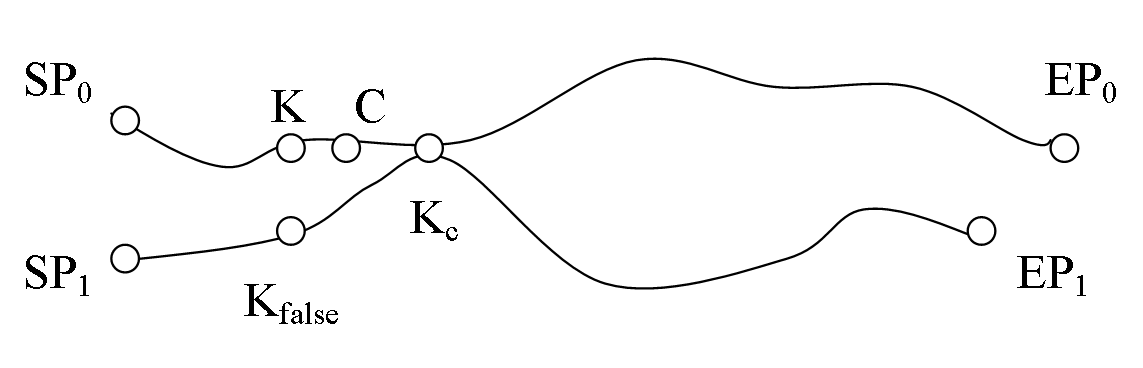
\includegraphics[width=4.5in]{./figures/collision-not-merge.PNG}
	\caption{Two chains which collide but do not merge}	
	\label{fig:collision-not-merge}
\end{figure}

\noindent \textit{\textbf{Solving the problem of collision.}} The inclusion of reduction function does not help in solving the problem of collision. Collisions still have the same effect if mapping function $F$ is used instead of encryption function $E$. But, if we use different reduction functions (hence, different mapping functions) for two colliding chains, the two chains do not merge and produce different keys from the colliding point $K_c$. Even though the ciphertext computed using $K_c$ is the same, different reduction functions in the two chains lead to different keys, thus preventing merging of the chains. Such a scenario is shown in figure \ref{fig:collision-not-merge}. As shown in the figure, the two chains end at different end points. As a result, the correct end point is retrieved from the hashtable during the attack phase and consequently the correct key is obtained. 


But practically, using $m$ different mapping functions for building the table has problems. Stamp and Low quote in \cite{stamp2007acb} that having $m$ mapping functions would make storing these functions very resource intensive, and thus that it's not a good idea. An apparent and more serious problem though, with having $m$ mapping functions, is that the attack phase would take a lot of time. During the attack phase, the given $C$ is evaluated for all the different mapping functions because the attacker does not know the chain in which $C$ appears. The attack time in such a case becomes proportional to $mt$. Hence, the idea of having different mapping function for each chain is not feasible. But, it provides a basis for the more practical table structure called the Hellman tables. 

\subsection{The practical TMTO attack}

The idea of using different mapping functions for two colliding chains is acceptable, but the downside of it is time-consuming attack phase. Based on various ideas gathered from the previous section, the idea of Hellman tables \cite{hellman1980ctm} is presented here. The two important features of Hellman tables are the following.

\begin{enumerate}
\item There are multiple tables in the precomputation, as compared to the previously considered one big table. The total number of tables is denoted by $r$. The main idea here is that each table has a different mapping function, and thus collision occuring among chains belonging to different tables do not result in a merge.

\item In order to reduce the possibility of collisions occuring among chains within same tables, the size of each table is restricted in accordance with the \emph{table stopping rule}. Hence the relation $mt^2$ = $2^n$ must hold.
\end{enumerate}

We describe in detail the precomputation and attack phase for the TMTO attack using the Hellman tables.\\
% need some thing more here.

\noindent \textit{\textbf{Precomputation phase.}} First, $r$ different random reduction functions are chosen, say \mbox{$R_1$, $R_2$, \ldots ,$R_r$}. Using each of these functions, $r$ tables are created in the same way as described for the ideal case. Each of the $r$ tables consist of $m$ chains with $t$ computations by using the mapping function $F$. Also, for each table, a different hashtable is created such that the starting and end points of the chains from a particular table are stored in the corresponding hashtable. 

\begin{figure}[ht!]
	\centering
		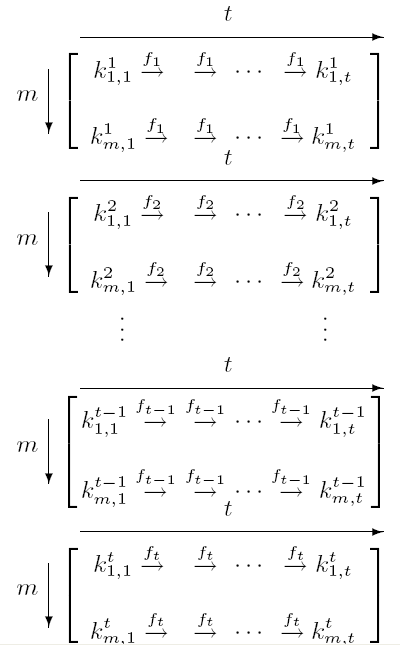
\includegraphics[width=3in]{./figures/hellman-tables.PNG}
	\caption{Hellman tables structure}	
	\label{fig:hellman-tables}
\end{figure}

The equations for creating the keys in the chain $i$ of table $j$ are shown below. The mapping function is denoted by $F_j$ and the reduction function by $R_j$.

\begin{align*}
& & K_{i,0} & = SP_i & & & &\\
1&. &K_{i,1} & = R_j(E_{K_{i,0}}(P)) & & & &\\
2&. &K_{i,2} & = R_j(E_{K_{i,1}}(P)) & & & &\\
& & &\vdots & & & &\\
(t-1)&. &K_{i,t-1} & = R_j(E_{K_{i,t-2}}(P)) & & & &\\
(t)&. &K_{i,t} & = R_j(E_{K_{i,t-1}}(P)) & & & &\\
& & EP_i & = K_{i,t} & & & &\\
\end{align*}

The time for precomputation is proportional to the number of computations that are done in all the tables, which is $mtr$. Hence, $P$ = $mtr$. Also, corresponding to each table, $m$ entries would exist in the hashtable. Hence, total number of entries in the hashtables is $mr$, resulting in required precomputation memory of an order $M$ = $mr$.\\

\noindent \textit{\textbf{Attack phase.}} During the attack phase, ciphertext $C$ is searched through each of the $r$ tables one by one. Let's consider the case in which $C$ is searched through a particular table $j$ which has the mapping function $F_j$ and reduction function $R_j$. 

First, $X$ is computed using the reduction function as, $X$ = $R_j(C)$. $X$ is then matched with the end points of the table. If $X$ matches with the end point $EP_{i,j}$ of the $i$'th chain, it means that the desired key lies in the $(t-1)$'th column of that chain. $SP_{i,j}$ is retrieved from the hashtable and $(t-1)$ computations are perfomed using $F_j$ to obtain the key in the $(t-1)$'th column, which we call $K_p$ for possible key. If the ciphertext derived using $K_p$ is the same as $C$, then $K_p$ is the key we are looking for. Otherwise, it is a case of false alarm. 

On the other hand, if $X$ does not match with any end point, $X$ is replaced with $F_j(X)$ and again matched with the end points. If there is a match, then the possible key appears in the $(t-2)$'th column. Just as before, $SP_{i,j}$ is retrieved from the hashtable and $(t-2)$ computations are performed of $F_j$ to obtain $K_p$. False alarm is checked for in the same way, which confirms if $K_p$ is the desired key or not. 

$X$ is iteratively replaced by $F_j(X)$ for a maximum of $(t-1)$ times, after which the same search is performed on the next table. If there is a match, and if it is not a false alarm, then the correct key is known and the attack is terminated. 

In the worst case, $K$ is found after searching through all the tables. Searching a single table requires the worst case of $t$ computations. Hence, the attack time is proportional to $rt$ in the worst case. This implies that the order of the attack time is $T$ = $rt$.\\

\noindent \textit{\textbf{Tradeoff equation.}} In order to derive the tradeoff equation, we repeat some of the important relations derived in this section. The first two relations are that for $M$ and $T$, 

\begin{center}
$M = mr$\\
$T = rt$\\
\end{center}

Then, we have the table stopping rule,
\begin{center}
$mt^2 = 2^k$\\
\end{center}

Further, it is required that all the possible keys are covered in the Hellman tables. Since the number of keys computed during the precomputation is $mtr$, we require

\begin{align*}
mtr = 2^k
\end{align*}

From the last two equations, we have $r$ = $t$. Hence, the number of tables is equal to the length of each chain. Eliminating $m$ and $t$ from the relations for $M$ and $T$, we get the following tradeoff equation

\begin{align*}
M^{2}T = 2^k
\end{align*}

% NEEDED - compare hellman tables with precomputed key tables - argue that hellman tables does not reduce precomputation time, but it does reduce memory requirement

\section{Hellman tables for stream ciphers}

Hellman tables for block ciphers have been used for mounting TMTO attacks on stream ciphers by Biryukov and Shamir in \cite{biryukov2000ctm}. Stream ciphers have a different working principle than block ciphers, and thus certain modifications in the original Hellman tables are proposed in order to apply them on stream ciphers. 

The Hellman tables for block ciphers are prepared using the plaintext $P$, which is assumed to be known to (or chosen by) the attacker before the precomputation phase of the attack. Using the available ciphertext $C$, the attacker can find the secret key $K$ if and only if $P$ is the plaintext that is used in constructing the tables. Hence in a way, the tables are \emph{static} and cannot be re-used if a different plaintext and ciphertext pair for the same key are known. The tables can only be re-used if the same plaintext $P$ is later encrypted using a different key, say, during a different run of the protocol using the block cipher.

In addition, one of the important goals while constructing the tables for block ciphers is to cover all the possible keys. This is so because, a key can be found only when it is available in one of the tables. If the key does not exist, it can never be found as the ciphertext obtained using the key would not match in the tables. If the ciphertext matches, it would only turn out to be a key which gives the same ciphertext as the correct key. 

Tables for stream ciphers differ from those for block ciphers based on these grounds. Tables prepared for stream ciphers (as we have already seen in section \ref{sec:bg-attack}) are not bound to a particular plaintext. They are general tables with prefix to state mapping, and can be re-used any number of times for keystream from different keys. Once a match is found, the current state of the LFSR is determined and it is then reversed to obtain the initial state. After this, the specific initialization parameters are used in finding the key from the initial state.

Also, stream ciphers move through a number of internal states while generating the output keystream. If the attacker is able to find any one of these internal states, the initial state is recovered and thus the key. The attacker has knowledge of \emph{data}, which comprises of subsequences of the keystream or the prefix of each of the internal state that occurs while generating the keystream. Using this data, several attempts of matching the current state in the precomputed tables can be made, thus increasing the probability of finding the key. This flexibility is not available to an attacker breaking block ciphers, since the only data known there is the ciphertext $C$. 

Attacks taking into consideration the availability of data, in addition to time and memory, are called time-memory-data tradeoff attacks (or TMDTO attacks). As we can see, TMDTO attacks are particularly suited to stream ciphers as a long keystream is available. Whereas in the case of block ciphers, we always have $D$ = $1$ representing the only available data $C$. Further, we describe the precomputation and attack phase for a TMDTO attack on stream ciphers.\\

\noindent \textit{\textbf{Precomputation phase.}} While attacking stream ciphers, the unknown part always is the current internal state and the known part is the prefix of the state. Before we discuss how the tables are organized, it is important to consider the number of states that are required to be covered by the tables, in order to have a high probability of a match. We have two set of states here; one, the states covered in the tables (number of such states is $P$) and two, the states covered while generating the keystream (the number of such states is $D$). According to equation \ref{eq:bday-paradox2}, in order to have a high probablity of a common state existing between these two sets, the product of the size of these sets must be greater than or equal to the size of the state space. 

Using the relation, we have $PD$ $\geq$ $N$. If we ignore the greater than sign, we get the lower bound on $P$ and $D$, and we have $P$ = $N/D$. As compared to the tables for block ciphers, $P$ is reduced by a factor of $D$ for stream ciphers. According to \cite{biryukov2000ctm}, reduction in the number of precomputed states can be achieved by either reducing the number of states in each table, or by reducing the number of tables itself. From the relation $P$ = $mt$.$t$/$D$, either $mt$ must become $mt$/$D$ (thus reducing number of states in each table) or $t$ must become $t$/$D$ (thus reducing the number of tables). The authors argue that the former option is not a good idea. In that case, the tables would accomodate less states than the maximum states allowed in a table to prevent collisions. As a result, the latter option is chosen, and the number of tables is reduced by the factor $D$. This in turn creates a dependency between $t$ and $D$ such that $t \geq D$, as there should atleast be one table. In the section \ref{} we argue that this is not a good idea, and show how the dependency can be eliminated. But for the moment, we continue with this idea. 

Thus for the precomputation phase, we have $t$/$D$ tables, each having $m$ chains with $t$ states each. The chains start with a random state $S_{j,0}$ (denoted by $SP_j$) indicating the first element in the j'th chain. The prefix for the starting state is computed, and a reduction function applied on the prefix to give the next state $S_{j,1}$. The prefix function is represented by $Prefix$ and the reduction function by $R$. Then, we have the following relation,

\begin{align*}
S_{j,1} = f_i(S_{j,0}) = R_i(Prefix(S_{j,0}))
\end{align*}  

\begin{figure}[ht!]
	\centering
		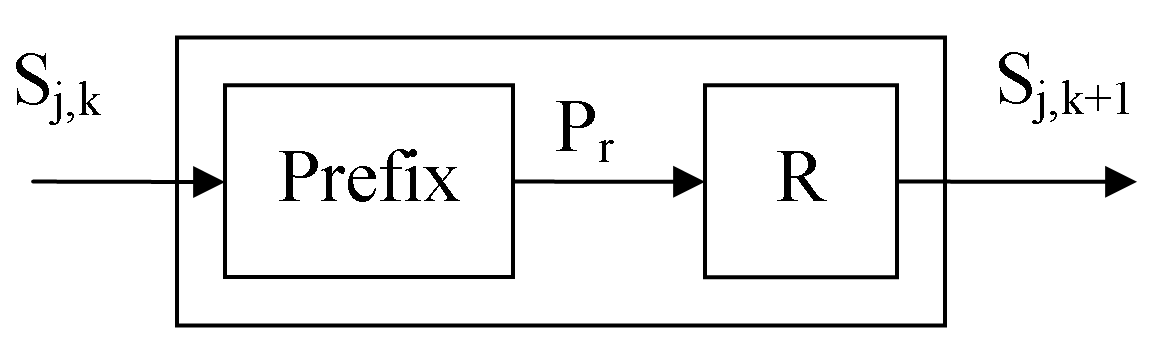
\includegraphics[width=3in]{./figures/mapping-function-stream.PNG}
	\caption{Mapping function for stream ciphers}	
	\label{fig:mapping-function-stream}
\end{figure}

The state $S_{j,1}$ is then used to compute $S_{j,2}$ and the process is repeated for $t$ such computations, at the end of which the last state $S_{j,t}$ is known. The mapping function $f_i$ is shown in the figure \ref{fig:mapping-function-stream} for such a transformation. The last state is referred to as end state and denoted by $EP_j$. In all, $m$ chains are created in this way as part of one table. The same is repeated for other tables but with different reduction functions, in order to avoid collision between different tables. 

The precomputation time $P$ for this phase is $mt^2/D$, as discussed before. Since the number of tables has reduced, the order of memory required to store the starting and end points of each chain also reduces. Hence we have, $M$ = $mt/D$.\\

\noindent \textit{\textbf{Attack phase.}} The attack phase for stream ciphers is similar to that for block ciphers. Every subsequence of the keystream is searched in all the tables. Each of the columns is checked for the possibility of the current state being present, and this repeated for each of the $t/D$ tables. In the worst case, the attack would require $t$ computations per table, for each prefix, which amounts to $t^2/D$ computations for each prefix. Hence the worst case attack time is of the order of $t^2$ and thus we have $T$ = $t^2$.\\

\noindent \textit{\textbf{Tradeoff equation.}} The tradeoff equation can be easily derived by eliminating the parameters $m$ and $t$ from the following three important equations,

\begin{align*}
M &= mt/D\\
T &= t^2\\
mt^2 &= N\\
\end{align*}

The tradeoff equation comes out to be,

\begin{align}
\label{eq:tmdto-hellman-stream} TM^2D^2 = N^2
\end{align}
  \\
\noindent \textit{\textbf{A general tradeoff equation.}} The tradeoff equation derived above is proposed in \cite{biryukov2000ctm} by Biryukov and Shamir. In the derivation of this equation, we have replaced the number of tables $r$ (the value of which is $t$ for block ciphers) with $r$ = $t/D$. The parameters $r$ and $t$ correspond to the precomputation phase whereas $D$ corresponds to the attack phase. Since the number of tables is such that $r \geq 1$, we have the condition that $D \leq t$. This creates a dependency of the attack phase parameter on the precomputation phase parameter. This dependency is particularly not helpful if we want to change $D$ frequently, for a fixed precomputation table. The precomputation phase in such a case would have to be carried out again with the new $D$ in consideration, before the attack could be mounted. 

Here, we describe a different and simpler form of the tradeoff equation, which uses the parameter $r$ in the precomputation phase without replacing it with $t/D$. Thus, if there are $r$ tables, with each table having $mt$ number of states, then the total number of states in the Hellman table structure is $mtr$. During the attack phase, $D$ states are traversed through, thus the product $mtr \times D$ must be $N$. Hence we have, 

\begin{align}
\label{eq:tmdto-hellman-general} mtr \times D = N
\end{align}

We call the equation \ref{eq:tmdto-hellman-general} as the general tradeoff equation for TMDTO attacks on stream ciphers using Hellman tables. Using this equation, the parameters $m$, $t$, $r$ and $D$ can be set independent of each other thus offering a greater flexibility while running the attack. Following these parameters, $T$ and $M$ can be calculated as follows.

\begin{align}
\label{eq:tmdto-hellman-general-memory} M &= mr\\
\label {eq:tmdto-hellman-general-time} T &= trD
\end{align}
 \\
In the next section results of the performance of Hellman tables for breaking HiTag2 are provided. The parameters used for these results are taken from the general tradeoff equation. Furthermore, the Biryukov and Shamir tradeoff equation is used for comparison with rainbow table in section \ref{sec:compare-hellman-rainbow}.

\section{Implementation and results}
\label{sec:hellman-table-impl}

The implementation of the Hellman tables for stream ciphers differs from the implementation of previously discussed TMTO attacks in certain ways. For every table a separate hashtable is constructed. This is because every table has its own reduction function. Each table is identified by a table number $i$ such that $1 \geq i \geq r$. The reduction function used for the table $i$ is shown in equation \ref{eq:reduction-function}, where $k$ represents a column in the chain $j$.

\begin{align}
\label{eq:reduction-function} S_{j,k+1} = f_i(S_{j,k}) = R_i(Prefix(S_{j,k})) = Prefix(S_{j,k}) \oplus i
\end{align}  

This ofcourse is a very simple reduction function and more complicated functions can be constructed. Though in the literal sense, this is not a reduction function since the input and output of the function are of same size which is 48 bits. This function is rather a permutation function and maps one element in the state space to another element in the same space. If prefixes of length 56 bits are used, then these 56 bits must be mapped to 48 bits of state. In this case, the terminology for the reduction function would be appropriate. But, we continue using the same name in the case of 48 bit prefixes in order to avoid creating new terms for special cases. 

The number of hashtables required is $r$ and the starting and end points of each table are stored in separate hashtables. In the implementation, we execute a separate program carry out the precomputation phase of the attack. This program computes the starting and end points for each table and stores them in an ASCII file on the local disk. The reason for doing this is that the precomputation takes hours to complete, for example for $P = 2^33$, the time taken is 13 hours. Hence, storing the tables in a file is a better idea instead of generating the precomputation tables each time the attack is executed.

The following steps are performed in sequence as part of the complete attack. 

\begin{enumerate}
\item The Hellman tables are created for given parameters $m,t,r$ and $D$, and stored in a file on the hard disk. This program is not part of the attack module.
\item The first step in the attack module is to prepare the hashtables by reading the file. The parameters from the file are matched with the parameters of the attack. If they are compatible then file reading process is continued. Otherwise the program terminates. The size of each hashtable prepared is $m$. The precomputation memory is as given by equation \ref{eq:tmdto-hellman-general-memory}. The time for precomputation $P$ is given by $mtr$.
\item Keystream is generated for the attack. The length of the keystream depends on value of $D$ chosen.
\item The attack is started. Each subsequence from the keystream is searched in the hashtable. The time for the attack is as given by equation \ref{eq:tmdto-hellman-general-time}. 
\end{enumerate}

The results of the attack for keys $K_1$ and $K_2$ are shown below. 

\begin{table}[ht!]
\begin{center}
\begin{tabular}{|c||c|c|c||c|c|c|}
\hline
Key & \multicolumn{3}{c||}{\textbf{$K_1$}} & \multicolumn{3}{c|}{\textbf{$K_2$}} \\ \hline \hline
M																				&	$2^{24}$ 	&	$2^{24}$ 	&	$2^{24}$ 	&	$2^{24}$ 	&	$2^{24}$ 	&	$2^{24}$ 	\\ 
t	  																		&	$2^{8}$ 	&	$2^{9}$ 	&	$2^{8}$ 	&	$2^{9}$		&	$2^{24}$ 	&	$2^{24}$ 	\\ 
r	  																		&	$2^{8}$ 	&	$2^{9}$ 	&	$2^{8}$ 	&	$2^{9}$		&	$2^{24}$ 	&	$2^{24}$ 	\\ 
D	  																		&	$2^{16}$ 	&	$2^{26}$ 	&	$2^{27}$ 	&	$2^{27}$	&	$2^{24}$ 	&	$2^{24}$ 	\\ \hline \hline
P	  																		&	$2^{32}$ 	&	$2^{33}$ 	&	$2^{32}$ 	&	$2^{33}$	&	$2^{24}$ 	&	$2^{24}$ 	\\ \hline
T	  																		&	$2^{31}$ 	&	$2^{32}$ 	&	$2^{31}$ 	&	$2^{32}$	&	$2^{24}$ 	&	$2^{24}$ 	\\ \hline
Precomputation time for file (hours)		&	6 	 			&	12 				&	6					&	12 				&	6					&	12				\\ \hline
Time for preparing hashtable (seconds)	&	158				&	 					& 116				&	116				&	6					&	12				\\ \hline
Number of times false key is found			&	2 				&	0 				&	3 				&	3 				&	6					&	12				\\ \hline
Number of times correct key is found 		&	2 				&	 					&	3 				&	1 				&	6					&	12				\\ \hline
Number of false alarms									&	139				&	0 				&	120				&	256				&	6					&	12				\\ \hline
Time for attack	(hours)									&	2.25 			&	0 				&	2.56 		 	&	5.12 			&	6					&	12				\\ \hline
\end{tabular}
\end{center}
\caption{Results of TMDTO Hellman attack for keys $K_1$ and $K_2$}
\label{tab:hellman-attack-results}
\end{table}

